\documentclass{beamer} %[handout]
%\usepackage{listings}
%\usepackage{textcomp}
%\usepackage{units}
%\usepackage{tikz}

%\usetikzlibrary[shapes,snakes, positioning]

\usepackage{color}
\usepackage{picture}
\usepackage{graphicx}

%%\usetheme{Malmoe}
\usetheme{metropolis} %%%
\metroset{block=fill}
\setbeamercolor{alerted text}{ fg=red!65!black}
%\setbeamertemplate{itemize items}[default]
%\setbeamertemplate{enumerate items}[default]
\setbeamercovered{transparent=50}
%\setbeamercovered{still covered={\opaqueness<1->{0}},again covered={\opaqueness<1->{35}}}
\setbeamertemplate{footline}{\hfill \insertframenumber/\inserttotalframenumber ~~~}

%\setbeamertemplate{bibliography entry title}{}
%\setbeamertemplate{bibliography entry location}{}
%\setbeamertemplate{bibliography entry note}{}


%\usepackage[natbib=true, bibstyle=authoryear, citestyle=authoryear-comp, backend=bibtex]{biblatex}
%\usepackage{natbib}
\usepackage{bibentry}
\nobibliography*
%\bibpunct[:]{(}{)}{,}{a}{}{,}
%\usepackage[ngerman]{babel}
\usepackage[T1]{fontenc}
    \usepackage[latin1]{inputenc}
    \usepackage{lmodern} 


\usepackage{amsmath}
\usepackage{amsthm}
\usepackage{amssymb}
\usepackage{hyperref}
\usepackage[T1]{tipa}
\usepackage{gb4e}
\usepackage{tikz}
\usepackage{marvosym}

\usetikzlibrary{trees}
\usetikzlibrary{matrix}
\newcommand{\citeposs}[2][]{\citeauthor{#2}'s (\citeyear[#1]{#2})}
\newcommand{\valueof}[1]{$\llbracket${\em #1}$\rrbracket$} 
%\newcommand{\valueof}[1]{$[[${\em #1}$]]$} 
%\newcommand{\mvalueof}[1]{$[[$ #1 $]]$} 
\newcommand{\mvalueof}[1]{\llbracket#1\rrbracket}
\newcommand{\vFill}{\vskip0pt plus 1filll}
\newcommand{\hFill}{\hskip0pt plus 1filll}
\newcommand{\bibj}[1]{$\cdot$ \bibentry{#1}\\}
%	\newcommand{\argmax}[1]{\underset{#1}{\operatorname{arg}\,\operatorname{max}}\;}

\newcommand{\tuple}[1]{\ensuremath{\left\langle #1 \right\rangle}}
\def\<{\langle}
\def\>{\rangle}
\def\jg#1{\leavevmode\llap{#1}}
\def\bad{\leavevmode\llap{*}}
\newcommand{\mdef}{\buildrel \text{d{}ef}\over =}
\newcommand{\light}[1]{\textcolor{grey}{#1}}

\newcommand*{\defeq}{\mathrel{\vcenter{\baselineskip0.5ex \lineskiplimit0pt
                     \hbox{\scriptsize.}\hbox{\scriptsize.}}}%
                     =}
%\renewcommand*{\bibfont}{\scriptsize}

\setbeamerfont{bibliography item}{size=\tiny}
\setbeamerfont{bibliography entry author}{size=\tiny}
\setbeamerfont{bibliography entry title}{size=\tiny}
\setbeamerfont{bibliography entry location}{size=\tiny}
\setbeamerfont{bibliography entry note}{size=\tiny}
\DeclareMathOperator*{\argmax}{arg\,max}
\DeclareMathOperator{\argmaxL}{arg\,max}


%%%%%%%%%%%%%%%%%%%%% Headling deletion%%%%%%%%%%%%%%%%%%%%%
\makeatletter
    \newenvironment{withoutheadline}{
        \setbeamertemplate{headline}[default]
        \def\beamer@entrycode{\vspace*{-\headheight}}
    }{}
\makeatother
%%%%%%%%%%%%%%%%%%%%%%%%%%%%%%%%%%%%%%%%%%%%%%%%%%%%%%%%%%%%
\beamertemplatenavigationsymbolsempty
%%%%%%%%%%%%%%%%% Block color%%%%%%%%%%%%%%%%%%%%%%%%%%%%%%
\definecolor{mygreen}{cmyk}{0, 1, 1, 0.5} %{0.82,0.11,1,0.25} 
\setbeamertemplate{blocks}[rounded][shadow=false]
\addtobeamertemplate{block begin}{\pgfsetfillopacity{0.8}}{\pgfsetfillopacity{1}}
\setbeamercolor{structure}{fg=mygreen}
\setbeamercolor*{block title example}{fg=blue!50,
bg= blue!10}
\setbeamercolor*{block body example}{fg= blue,
bg= blue!5}

%%%%%%%%%%%%%%%%%%%%%%%%%%%%%%%%%%%%%%%%%%%%%%%%%%%%%%%%%%

%%%%%%%%%%%%%%%%%%%% Numbering%%%%%%%%%%%%%%%%%%%
\resetcounteronoverlays{exx}
%%%%%%%%%%%%%%%%%%%%%%

%%%%%%%%%%%%%% Appendix %%%%%%%%%%%%%%%%%%%%%

%%%%%%%%%%%%%%%%%%%%%%%%%%%%%%%%%%%%%%

\begin{document}
\renewcommand{\inserttotalframenumber}{27}
\title{Learning biases may prevent the lexicalization of pragmatic inferences}%\\[0,1cm] 
\subtitle{A case study combining iterated learning and\\ replicator dynamics }
%\subtitle{An overview}

\author{\center Thomas Brochhagen\\ILLC, University of Amsterdam\\
{\tiny Joint work with Michael Franke (T\"ubingen) \& Robert van Rooij (Amsterdam)}}
%\author{\center Thomas Brochhagen\inst{1} \and Michael Franke \inst{2} \and Robert van Rooij \inst{1}}
%\institute{\inst{1} ILLC, University of Amsterdam \and \inst{2} Department of Linguistics, University of T\"ubingen\vspace{1cm}}
 %{../../03orga+misc/logos+graphics/essence_logo.png}

\date{\center \scriptsize Centre for Language Evolution seminar series, Edinburgh, 2016.07.19}

%%%%
\metroset{sectionpage=none}
\begin{frame}
\titlepage
\end{frame}
%
%%\begin{withoutheadline}
%\begin{frame}
%\tableofcontents
%\end{frame}
%\end{withoutheadline}
\begin{withoutheadline}

\section{Introduction}
\begin{frame}
	\frametitle{The semantics-pragmatics distinction}
	\alert{Semantics}\\ Literal meaning (truth-conditional)\\ \vspace{2cm}
	\alert{Pragmatics}\\ Information beyond literal meaning (e.g. defeasible inferences)

\end{frame}
\begin{frame}
	\frametitle{Scalar inferences}
%\vspace{1cm}
\begin{exe}
\itemsep1em
\item \tuple{few, \alert{some}, many, most, \alert{all}}\\ \begin{xlist} \itemsep1em
	\item All students came to class\\ $\rightarrow$ \alert{Some} students came to class
	\item Some students came to class\\ $\leadsto$ \alert{Not all} students came to class
	\end{xlist}
\item \tuple{may, should, must}
\item \tuple{one,two,three, ...}
\item \tuple{or, and}
\item ...
\end{exe}

\end{frame}

\begin{frame}
  \begin{center}
	  The use of a less informative expression when a more informative one \underline{could have been used}^{\bf{\alert{*}}} can license a defeasible inference that the stronger alternatives do not hold
  \end{center}

\vspace{3cm}

\noindent {\bf \alert{*}}The hearer assumes the addressee to be knowledgeable and cooperative

\vFill

\begin{block}{}
	{\tiny \bibj{horn:1972} \bibj{gazdar:1979} \bibj{grice:1975}}
\end{block}
\end{frame}

\begin{frame}
  \frametitle{Explanations for a lack of semantic upper-bounds I}
 \begin{center}
  (1) Signal no commitment to stronger alternatives when knowledge/cooperativity are not given
  \end{center}

Cf. lexicalizing `some' and `sbna'

Conditions that may pressure for English-like semantics:
\begin{itemize}
  \item Contextual cues are very reliable
  \item Morphosyntactic disambiguation is not frequently necessary
  \item Morphosyntactic disambiguation is not very costly 
  \item Cost of larger lexica higher than morphosyntactic disambiguation
\end{itemize}
\end{frame}

\begin{frame}
  \frametitle{Explanations for a lack of semantic upper-bounds II}
\begin{center}
    (2) Lack of upper-bounds provides learnability advantage
\end{center}

\end{frame}

\begin{frame}

  \begin{enumerate}
	  \item Why are (pragmatically inferred) upper-bounds of weak(er) alternatives not part of semantics? \label{des-1}
	  \item What justifies semantic structure in light of pragmatic enrichment? \label{des-2}
  \end{enumerate}
\pause
  \vspace{2cm} 
Today's talk:
  \begin{itemize}
	  \item Propose a model to address (\ref{des-2}) and analyze dynamics of linguistic pressures more broadly
	  \item Use (\ref{des-1}) as a case study for (\ref{des-2}) 
  \end{itemize}
\end{frame}
\metroset{sectionpage=progressbar}


\section{Model}
\begin{frame}
	\frametitle{Components I: Cultural transmission}

Two competing pressures:
\vspace{0,5cm}
\begin{enumerate} \itemsep1em
	\item Communicative efficiency\\[0,3cm] ... as replicator dynamics 
	\item Learnability \\[0,3cm] \makebox(0,0){\put(155,8.9\normalbaselineskip){%
               $\left.\rule{0pt}{4.5\normalbaselineskip}\right\}$ Replicator-mutator dynamics }}
	... iterated Bayesian learning\\ \hspace{0.47cm} as mutator dynamics
		\end{enumerate}
%\vspace{1cm}
%\begin{enumerate}
%	\item Functional pressure: Replicator(-mutator) dynamics 
%	\item Learnability: iterated Bayesian learning (mutation)
%\end{enumerate}
\vFill
\begin{block}{}
	{\tiny \bibj{griffiths+kalish:2007} \bibj{hofbauer+sigmund:2003} \bibj{nowak+krakauer:1999}}
\end{block}
\end{frame}

\begin{frame}
	\frametitle{Components II: Probabilistic (pragmatic) language users}
	\vspace{1cm}
\begin{itemize}\itemsep2em
	\item Varied lexica 
	\item Varied production and comprehension behavior \makebox(0,0){\put(0,5\normalbaselineskip){%
               $\left.\rule{0pt}{3.5\normalbaselineskip}\right\}$ A player's type}} \\
	(here: parametrized {\em literal} or {\em pragmatic}) 
\end{itemize}

\vFill
\begin{block}{}
	{\tiny \bibj{benz+etal:2005} \bibj{bergen+etal:2016} \bibj{frank+goodman:2012} \bibj{franke+jaeger:2014}}
\end{block}
\end{frame}

\begin{frame}
	\frametitle{Lexica}
	\begin{itemize}
		\item $s_1$: Bill read some but not all books
		\item $s_2$: Bill read all books
	\end{itemize}
\vspace{1cm}

\begin{centering}
	 $L_a$ = \bordermatrix{~ & m_{\text{all}} & m_{\text{some}} \cr 
                  s_1 & 0 & 1 \cr
s_2 & 1 & 1 \cr}\\[1.5cm]
\end{centering}

\begin{centering}
	$L_b$ = \bordermatrix{~ & m_{\text{all}} & m_{\text{some}} \cr 
	s_1 & 0 & 1 \cr
s_2 & 1 & 0 \cr}\\
\end{centering}

\end{frame}

\begin{frame}
	\underline{Literal behavior} 	
\begin{flalign}
&R_{0}(s|m;L) \propto P^*(s) L_{sm}\label{litl}\\
&S_{0}(m|s;L) \propto \text{exp}(\lambda \; L_{sm}) \label{lits}
\end{flalign}
\underline{Pragmatic behavior}
\begin{flalign}
&R_{1}(s|m;L) \propto P^*(s) S_{0}(m|s;L) \label{pragl}\\
&S_{1}(m|s;L) \propto  \text{exp}(\lambda \; R_{0}(s|m;L)^\alpha) \label{prags}
\end{flalign}
~\\
%\vspace{1cm}
%\begin{itemize}
%	\item Soft-max parameter $\lambda > 0$
%	\item pragmatic violations parameter $\alpha \in [0,1]$
%	\item $P^* \in \Delta(S)$
%\end{itemize}
\vspace{1cm}
{A \alert{player type} $t_i$ is a combination of signaling behavior and a lexicon}
\end{frame}

\begin{frame} 
	\frametitle{Functional pressure (replicator dynamics)}
	\begin{itemize}\itemsep1.5em
			\item Population of types $x$\\[0,3cm] $x_i$ is the proportion of $t_i$ in $x$
			\item Fitness of type $i$\\[0,3cm] $f_i =  \sum_j x_j U(x_i,x_j)$
			\item Average fitness in the population\\[0,3cm] $\Phi = \sum_i x_i f_i$
	\end{itemize}
\end{frame}

\begin{frame}
	\frametitle{Iterated learning (mutator dynamics)}
\begin{itemize} \itemsep1em
		\item $Q_{ji} \propto \sum_d P(d|t_j)P(t_i|d)$
		\item $d = \tuple{\tuple{s_h,m_n}, ..., \tuple{s_l,m_o}}$ of length $k$
		\item $P(d|t_j)$ corresponds to $t_j$'s production probabilities of
		\item $P(t_i|d) \propto [P(t_i)P(d|t_i)]^l$, $l \geq 1$
		\item Prior encodes learning biases of players prior to data exposure\\[0,3cm]
		      $P(t_i) \propto n - c \cdot r$, where $n = |S|$ and $r$ a count of semantically upper-bounded weak alternatives in $L_i$
\end{itemize}
\end{frame}

\begin{frame}
	\frametitle{Parametrized posterior $P(d|t_i)^l$}
\begin{itemize}\itemsep2em
	  \item $l = 1$ corresponds to posterior sampling
	  \item $l \to \infty$ approaches MAP
	\end{itemize}
\end{frame}


\section{Analysis}



\begin{frame}
	\frametitle{Lexica, signaling behavior \& types}
\underline{Lexica}
\begin{table}
\centering 
\begin{tabular}{l c l}
$L_1$ = $\begin{pmatrix} 0 & 0 \\ 1 & 1 \end{pmatrix}$ & 
$L_2$ = $\begin{pmatrix} 1 & 1 \\ 0 & 0 \end{pmatrix}$ & 
$L_3$ = $\begin{pmatrix} 1 & 1 \\ 1 & 1 \end{pmatrix}$\\[1cm]

$L_4$ = $\begin{pmatrix} 0 & 1 \\ 1 & 0 \end{pmatrix}$ &
$L_5$ = $\begin{pmatrix} 0 & 1 \\ 1 & 1 \end{pmatrix}$ &
$L_6$ = $\begin{pmatrix} 1 & 1 \\ 1 & 0 \end{pmatrix}$
\end{tabular}
\end{table}
\underline{Signaling behavior}\\ {\em Literal} or {\em pragmatic}\\[0.75cm]
\underline{Types}\\ $12$ types ($2$ behaviors $\times$ $6$ lexica)
\end{frame}

\begin{frame} 
\begin{center}What factors lead to the selection of $L_5$-like semantics?\end{center}
\end{frame}

\begin{frame}
\frametitle{Fitness only}
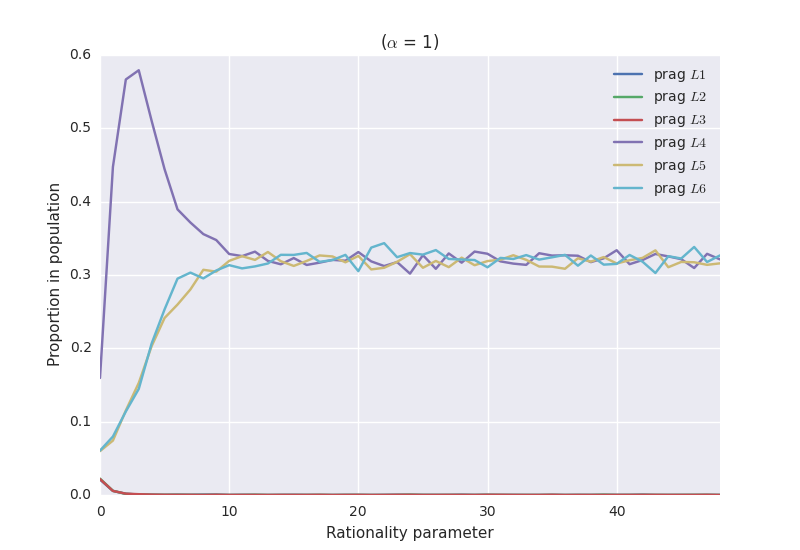
\includegraphics[width=\linewidth,height=\textheight,keepaspectratio]{07fitness}

\end{frame}

\begin{frame}
\frametitle{Learning only}
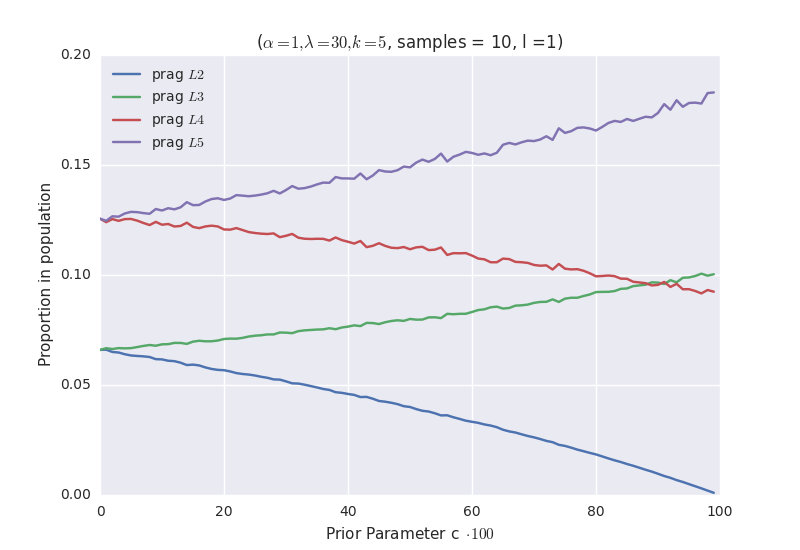
\includegraphics[width=\linewidth,height=\textheight,keepaspectratio]{07learning}

\end{frame}

\begin{frame}
	\frametitle{Fitness and learning}

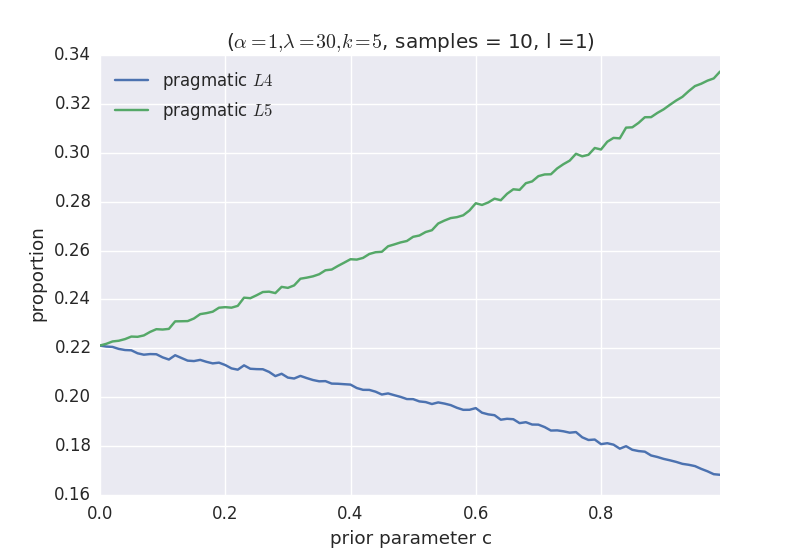
\includegraphics[width=\linewidth,height=\textheight,keepaspectratio]{03cost-with-l1}

\end{frame}

\begin{frame}
  \frametitle{Interim remarks}
  \begin{itemize}
	\item Lack of semantic-upper bounds can overcome pressures and stabilize in a population provided...
	  \begin{itemize}
		\item Bias for simpler representations
		\item Pragmatics to compensate lack of upper-bounds in use
	  \end{itemize}
%	\item Weak learning bias sufficient for selection of $L_5$ over $L_5$ (and the latter's incumbency)
  \end{itemize}
\pause
  But

  \begin{itemize}
    \item Highly polymorphic populations even for high $c$
    \item Role of learning mechanisms, rationality, and learning observations unexplored
  \end{itemize}

\end{frame}

\begin{frame}
	\frametitle{Effect of prior with more posterior maximization}
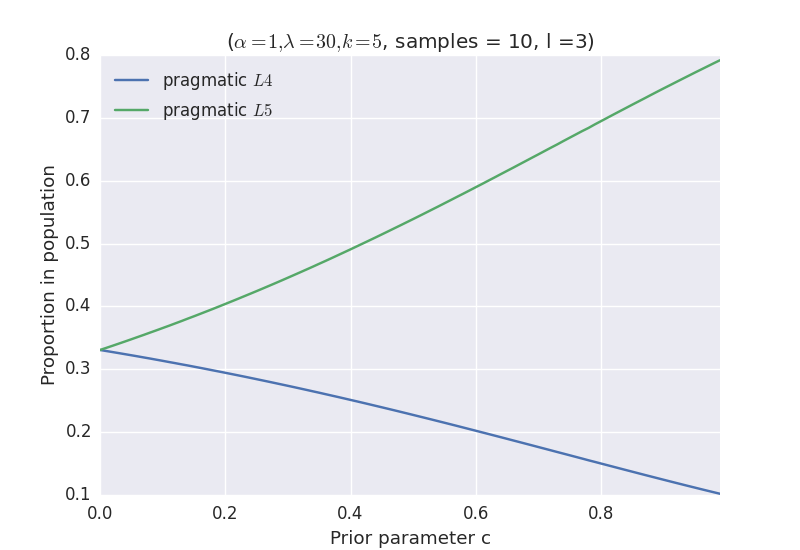
\includegraphics[width=\linewidth,height=\textheight,keepaspectratio]{02cost-with-l3}

\end{frame}

\begin{frame}
	\frametitle{Prior and posterior}

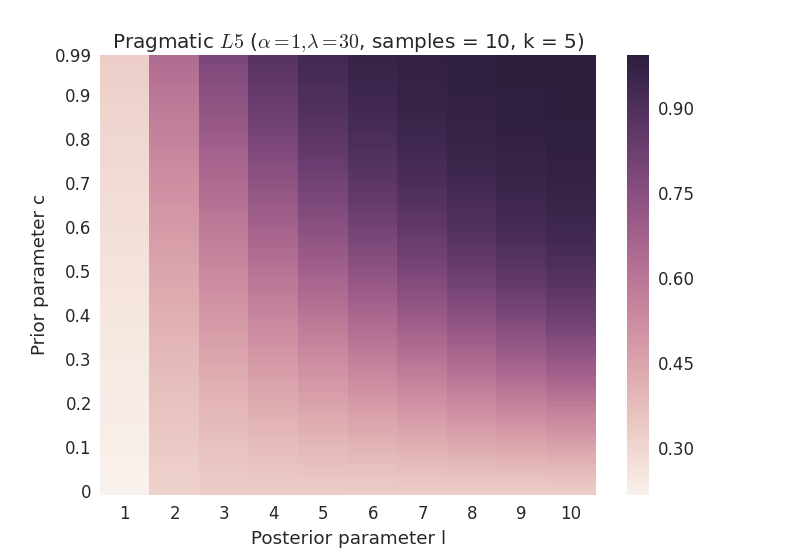
\includegraphics[width=\linewidth,height=\textheight,keepaspectratio]{01heatmap}

\end{frame}

\begin{frame}
  \frametitle{Rationality and sequence length I}
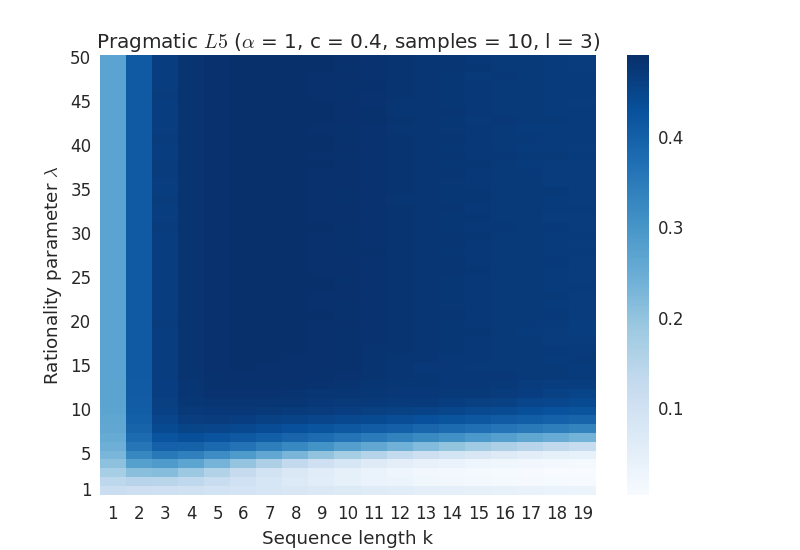
\includegraphics[width=\linewidth,height=\textheight,keepaspectratio]{05heatmap}
\end{frame}

\begin{frame}
  \frametitle{Rationality and sequence length II}
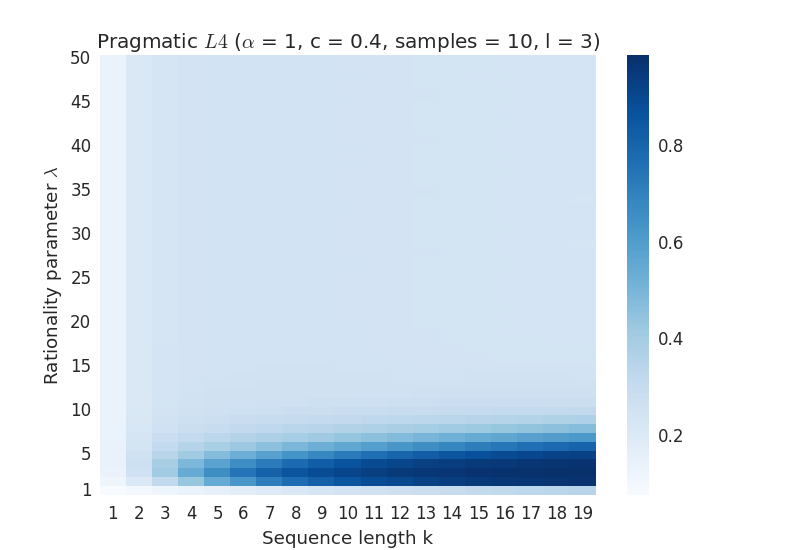
\includegraphics[width=\linewidth,height=\textheight,keepaspectratio]{06heatmap}
\end{frame}


\section{Conclusion \& Outlook}
\begin{frame}
  \frametitle{Concluding remarks: Application}
  \begin{itemize}
		\item Learnability steers language\\ towards simpler semantics
		\item Pragmatics compensates for \makebox(0,0){\put(0,4\normalbaselineskip){%
               $\left.\rule{0pt}{2.5\normalbaselineskip}\right\}$ Lack of semantic upper-bounds}} \\
 potential loss in expressivity  
		\item Functional advantages 
		\begin{itemize}
		  \item Reliability of contextual cues to cancel implicatures
		  \item Lexicon size
		  \item ...
		\end{itemize}
 \end{itemize}

Provided

\begin{itemize} 
  \item Some degree of rationality in learning \& choice
  \item Relation between bounds and simplicity
\end{itemize}
\end{frame}

\begin{frame}
	\frametitle{Concluding remarks: Model}
\begin{itemize}\itemsep1em
		\item Combines 
		  \begin{itemize} 
		    \item Functional pressure
		    \item Learning pressure 
		    \item (Probabilistic) hearer \& speaker models
		    \item Distinct languages
		  \end{itemize}
	\end{itemize}
\end{frame}

\begin{frame}
  \frametitle{Future directions}
    \begin{itemize}\itemsep1em
      \item Generalization
      \item Frequency effects
      \item Larger lexica \& uncertainty
      \item Further applications
    \end{itemize}
\end{frame}
%%%%%%%%%%%%%%%%%%%% BIBLIOGRAPHY%%%%%%%%%%%%%%%%%%%%%%%%%%%%%%%%%%%%%%%
\section[References]{References}
\begin{frame}[allowframebreaks]\frametitle{References}
\tiny
\setbeamertemplate{bibliography item}[text]
%\begin{multicols}{2}
\bibliographystyle{alpha} %
\bibliography{./../paper/bounds-rmd}
%\end{multicols}
\end{frame}
\end{withoutheadline}
%%%%%%%%%%%%%%%%%%%%%%%%%%%%%%%%%%%%%%%%%%%%%%%
\end{document}

